\documentclass{beamer}
% \usepackage{animate}
\usepackage{multimedia}
\usepackage[english,russian]{babel}

\usepackage{pgfpages}
\setbeameroption{show notes on second screen}
%https://tug.ctan.org/macros/latex/contrib/beamer/doc/beameruserguide.pdf

\usepackage[T2A]{fontenc}
\usepackage[utf8]{inputenc}

\setbeamertemplate{caption}[numbered]

\usetheme{CambridgeUS}
\usecolortheme{dolphin}


\title[Commands Vulkan API]{Работа с командами в Vulkan API}
\author[Быковских Д.А.]{Быковских Дмитрий Александрович}
\date{12.10.2024}

\begin{document}
	\begin{frame}
		\titlepage
	\end{frame}
	%\section{Обзор}


	\begin{frame}{Содержание}
		\begin{itemize}
			\item Концептуальная модель Vulkan API
			\item Объекты Vulkan API
			\item Очередь (Queue)
			\item Буфер команд (Command Buffer) и пул команд (Command Pool)
			\item Команды (Commands)
			\item Синхронизация (Synchronization)
		\end{itemize}
	\end{frame}

	\begin{frame}{Концептуальная модель Vulkan API}
		Концептуальная модель Vulkan API представляет собой низкоуровневую архитектуру для работы с графическими и вычислительными задачами на GPU, предоставляя разработчикам прямой контроль над аппаратными ресурсами.

		\begin{figure}
			\href{https://sourceforge.net/projects/cpp-lects-rus/files/cpp-graduate/10-3dgraphics.pdf}{
				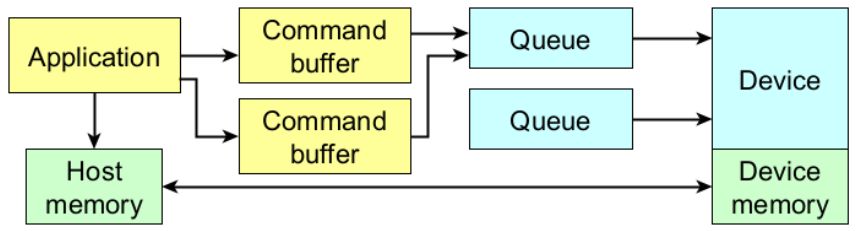
\includegraphics[width=0.95\textwidth]{images/Vulkan-model.png}}
			\caption {Схема концептуальной модели Vulkan API}
		\end{figure}

		\note{

			Особенности:
			\begin{itemize}
				\item 
				Высокий уровень параллелизма (Формирование буфера команд)
				\item 
				Асинхронность (Выполнение команд через очереди Queue)
				\item
				Явное (низкоуровневое) управление памятью (Host memory и Device memory) 
			\end{itemize}

		}


	\end{frame}

	\begin{frame}{Объекты Vulkan API}

		\begin{figure}
			\href{https://gpuopen.com/learn/understanding-vulkan-objects/}{
				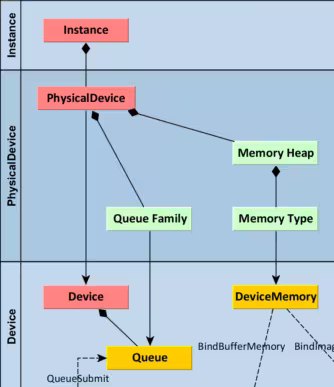
\includegraphics[width=0.45\textwidth]{images/VulkanObjects-short.png}}
			\caption {Часть схемы объектов Vulkan API}
		\end{figure}

		\note{
			Функции создания объектов
		\begin{itemize}
			\item 
			vkCreateInstance --- точка взаимодействия с драйвером (м.б. несколько)
			\item 
			vkEnumeratePhysicalDevices --- выбор физических устройств
			\item
			vkGetPhysicalDeviceQueueFamilyProperties --- выбор поддерживаемых типов очередей
			\item
			vkCreateDevice --- логическое устройство, с поддерживаемыми типами очередей, памятью и т.д.
			\item
			vkGetDeviceQueue --- дескриптор очереди для отправки команд на физической устройство через драйвер
		\end{itemize}
			
		}


	\end{frame}

	\begin{frame}{Очередь}{Queue}
		Очередь (queue) — это механизм для отправки команд от приложения на выполнение на графический процессор (GPU). 

		VkQueueFamilyProperties --- структура, описывающая свойства семейства очередей на конкретном физическом устройстве.

		Поля структуры:
		\begin{itemize}
				\item \texttt{queueFlags} --- флаги возможностей очереди (типы операций):
				\begin{itemize}
						\item \texttt{VK\_QUEUE\_GRAPHICS\_BIT} --- поддержка графических операций.
						\item \texttt{VK\_QUEUE\_COMPUTE\_BIT} --- поддержка вычислительных операций.
						\item \texttt{VK\_QUEUE\_TRANSFER\_BIT} --- поддержка операций передачи данных (копирование буферов и изображений).
						\item \texttt{VK\_QUEUE\_SPARSE\_BINDING\_BIT} --- поддержка операций с разреженными ресурсами.
						\item и др.
				\end{itemize}
				
				\item \texttt{queueCount} --- количество очередей, доступных в этом семействе.
		\end{itemize}

		\note{
			Поля структуры (продолжение)\\
			\begin{itemize}
			\item 
			\texttt{minImageTransferGranularity} --- минимальная единица передачи изображений (размеры элемента по X, Y и Z). Полезно для операций передачи изображения и использования разреженных текстур (sparse textures), где может понадобиться копировать данные с определённой минимальной единицей.
			\item
			\texttt{timestampValidBits} --- количество валидных битов в метках времени (timestamps). Если поддерживается, это число указывает, сколько битов будет использоваться для меток времени, полученных с помощью команд, вроде \texttt{vkCmdWriteTimestamp}.
			\item
			 и др.
			\end{itemize}
		}
			
		\end{frame}
	
	\begin{frame}{Буфер команд и пул команд} {Command Buffer and Command Pool}

		Пул команд (Command Pool) --- объект, который управляет выделением и освобождением памяти, предназначенной для командных буферов.

		Буфер команд (CommandBuffer) --- коллекция команд, которая отправляется в соответствующую очередь для обработки на GPU, затем они проверяются и компилируются с помощью драйвера.
		После компиляции буферы команд могут использоваться повторно.
		\\
		Виды командных буферов\\
		\begin{itemize}
			\item 
			Первичные помимо отправки команд в очередь, могут использовать вторичные буферы.
			\item 
			Вторичные не могут быть прямо отправлены в очередь.
		\end{itemize}
		
		\note{
			Примечания. \\
			1. Пул команд зависит от семейства очередей, позволяет многократно использовать эти командные буферы, что минимизирует накладные расходы на запись команд.
			
			2. Каждый буфер команд управляет своим состояниями независимо.
			\\
			Существует три состояния буфера команд:
			\begin{itemize}
				\item Начальное состояние (до записи или при сбросе)
				\item Состояние записи (между вызовами vkBeginCommandBuffer и vkEndCommandBuffer)
				\item Состояние выполнения (отправка на выполнение)
			\end{itemize}
		}
		

	\end{frame}

	\begin{frame}{Команды}{Commands}
		В Vulkan API существуют несколько типов командных буферов, которые могут быть использованы для записи и исполнения различных команд.

		Категории команд
		\begin{itemize}
			\item 
			Команды управления памятью (копирование, заполнение/очистка, обновление данных)
			\item
			Графические команды (управление процессом рендеринга)
			\item
			Команды управления состоянием (управление наборами дескрипторов, привязка конвейеров и проходов)
			\item
			Команды синхронизации (синхронизация памяти и кэширование между командами; установка, ожидание и сброс сигналов события)
			\item
			и др.
		\end{itemize}

	\end{frame}

	\begin{frame}{Синхронизация}{Synchronization}

		Vulkan предоставляет несколько механизмов для синхронизации выполнения команд между очередями и/или внутри одной очереди. \\
		Механизмы синхронизации:
		\begin{itemize}
			\item
			Блокирующие функции (vkDeviceWaitIdle и vkQueueWaitIdle) --- приостанавливает работу приложения (потока) и ожидает завершения всех задач (команд) на всех очередях устройства и в конкретной очереди соответственно.
			\item
			Заборы (Fences) --- используются для синхронизации между CPU и GPU.
			\item 
			Семафоры (Semaphores) --- применяются для синхронизации между очередями (например, через сигналы).
			\item
			События (Events) --- используются для синхронизации выполнение команд внутри одной очереди.
			\item
			Барьеры (Barriers) --- применяются для синхронизации доступа к ресурсам (например, буферам и изображениям и т.д.).
		\end{itemize}

		\note {
		
		Выполнение команд в происходит через очереди. \\
		Вообще говоря команды выполняются асинхронно. \\
		Команды могут быть различной сложности, а следовательно длиться разное количество времени. 

		}

	\end{frame}

\if 0
\begin{columns}
	
	\begin{column}{0.5\textwidth}
		\begin{itemize}
			\item
			
		\end{itemize}
	\end{column}
	\begin{column}{0.5\textwidth}
		\begin{itemize}
			\item
		\end{itemize}
	\end{column}
	
\end{columns}
\fi
	
\end{document}
